\chapter{Implementacija i korisničko sučelje}
		
		
		\section{Korištene tehnologije i alati}
		
			\textbf{\textit{dio 2. revizije}}
			
			 \textit{Detaljno navesti sve tehnologije i alate koji su primijenjeni pri izradi dokumentacije i aplikacije. Ukratko ih opisati, te navesti njihovo značenje i mjesto primjene. Za svaki navedeni alat i tehnologiju je potrebno \textbf{navesti internet poveznicu} gdje se mogu preuzeti ili više saznati o njima}.
			 		
			\eject 
		
	
		\section{Ispitivanje programskog rješenja}
			
			\subsection{Ispitivanje komponenti}
			\textit{Potrebno je provesti ispitivanje jedinica (engl. unit testing) nad razredima koji implementiraju temeljne funkcionalnosti. Razraditi \textbf{minimalno 6 ispitnih slučajeva} u kojima će se ispitati redovni slučajevi, rubni uvjeti te izazivanje pogreške (engl. exception throwing). Poželjno je stvoriti i ispitni slučaj koji koristi funkcionalnosti koje nisu implementirane. Potrebno je priložiti izvorni kôd svih ispitnih slučajeva te prikaz rezultata izvođenja ispita u razvojnom okruženju (prolaz/pad ispita). }
			
			
			
			\subsection{Ispitivanje sustava}
			
			  Ispitivanje smo proveli koristeći Selenium WebDriver unutar JUnit testova. Cilj ispitivanje bio je provjera nekih glavnih funkcionalnosti sustava i pronalazak pogrešaka. WebDriver potrebno je instalirati lokalno na računalo i prilikom pokretanja postaviti putanju koja se nalazi u varijablama okruženja sustava. Prilikom testiranja aplikacija se pokretala na lokalnom računalu zato što je Heroku servis na kojemu je aplikacija puštena u pogon dosta sporiji, pa bi testovi trajali nešto dulje vremena.
			  Slika testova koji su se uspješno izvršili i na aplikaciji puštenoj u pogon na servisu Heroku će biti priložena.\\
	
		 	\textbf{\textit{Ispitni slučaj 1: Prijava planinara u sustav s ispravnim/neispravnim podacima}}
		 	
		 	\begin{lstlisting}
		 	public void testLoginBadAndGoodCreds() throws InterruptedException {
		 		//Driver setup...
		 		System.setProperty("webdriver.chrome.driver", "/path...");
		 		WebDriver driver = new ChromeDriver(); 
		 		driver.manage().timeouts().implicitlyWait(Duration.of(20, ChronoUnit.SECONDS));
		 		
		 		driver.get("http://localhost:3000/home");
		 		WebElement loginButton = driver.findElement(By.id("log-button"));
		 		loginButton.click();
		 		String loginUrl = driver.getCurrentUrl();
		 		assertTrue(loginUrl.contains("/login"));
		 		WebElement Emailelement = driver.findElement(By.id("email"));        
		 		Emailelement.sendKeys("luka.ravenscak");   
		 		WebElement passElement = driver.findElement(By.id("password"));
		 		passElement.sendKeys("password");
		 		driver.findElement(By.className("submitButton")).click();
		 		WebElement element = driver.findElement(By.className("errorText"));
		 		assertEquals("Neispravan oblik mail-a.", element.getText());
		 		Emailelement.clear();
		 		Emailelement.sendKeys("luka.ravenscak@fer.hr");
		 		passElement.clear();
		 		passElement.sendKeys("mypassword");
		 		driver.findElement(By.className("submitButton")).click();
		 		element = driver.findElement(By.id("error-span"));
		 		assertEquals("Neispravan e-mail ili lozinka.", element.getText());
		 		passElement.clear();
		 		passElement.sendKeys("password");
		 		driver.findElement(By.className("submitButton")).click();
		 		Thread.sleep(1000);
		 		assertTrue(driver.getCurrentUrl().contains("/mountaineering-community"));
		 		
		 		driver.quit();
		 	}
		 	\end{lstlisting}
	 	
	 	 U 1. ispitnom slučaju ispitana je funkcionalnost prijave u sustav. Prvo se dohvati početna stranica aplikacije te se odabire opcija "Prijavi se" koja se nalazi na zaglavlju stranice. Zatim se unese neispravni oblik email-a, na što aplikacija vraća obavijest "Neispravan oblik mail-a.", nakon toga se unose valjani email i neispravna lozinka, aplikacija reagira tako da vrati obavijest "Neispravan e-mail ili lozinka.". Na kraju se unesu ispravni podaci za prijavu i aplikacija reagira uspješnom prijavnom korisnika u sustav i odvede korisnika na stranicu vlastite planinarske zajednice.\newline
	 	 
	 		\textbf{\textit{Ispitni slučaj 2: Planinar pretražuje ostale korisnike}}
	 	
	 	\begin{lstlisting}
	 		public void testSearchAdminOnAllUserSearchPage() throws InterruptedException {
	 			
	 			//Driver setup
	 			driver.get("http://localhost:3000/login");
	 			
	 			WebElement element = driver.findElement(By.id("email"));        
	 			element.sendKeys("luka.ravenscak@fer.hr");
	 			element = driver.findElement(By.id("password"));
	 			element.sendKeys("password");
	 			driver.findElement(By.className("submitButton")).click();
	 			Thread.sleep(2000);
	 			assertTrue(driver.getCurrentUrl().contains("/mountaineering-community"));
	 			
	 			WebElement searchAllButton = driver.findElement(By.className("search-all-button"));
	 			searchAllButton.click(); 
	 			
	 			assertTrue(driver.getCurrentUrl().contains("/users/search"));    
	 			element = driver.findElement(By.name("searchText"));        
	 			element.sendKeys("admin");
	 			driver.findElement(By.name("searchText")).click();
	 			driver.findElement(By.className("all-user-photo")).click();
	 			Thread.sleep(2000);	    
	 			assertTrue(driver.getCurrentUrl().contains("/profile"));
	 			
	 			assertEquals("admin", driver.findElement(By.id("name-profile")).getAttribute("value"));
	 			driver.quit();
	 		}
	 	\end{lstlisting}
 	
	 	U 2. ispitnom slučaju ispitana je funkcionalnost pretrage svih korisnika od strane planinara. Prvo se provede prijava planinara u sustav, zatim prijavljeni korisnik odabire opciju "Pretraži sve planinare" te ga aplikacija preusmjeri na stranicu za pretragu svih korisnika. Korisnik u prostor za unos teksta za pretragu upiše "admin" i odabire opciju pretrage, aplikacija u rezultatima pretrage vrati traženog korisnika. Nakon toga korisnik odabere adminovu sličicu profila i aplikacija mu prikaže adminov profil. Testiranje je provedeno na način da se pretražuje profil admina, koji unutar aplikacije uvijek postoji.\newline
	 	
 		\textbf{\textit{Ispitni slučaj 3: Pretraga i arhiviranje posjećenog planinarskog doma}}
 		
 		\begin{lstlisting}
 			public void testMountainLodgeSearchArchiveAndBadgeAdd() throws InterruptedException {
 			//Driver setup
 			
 			driver.get("http://localhost:3000");
 			driver.findElement(By.className("domovi")).click();
 			assertTrue(driver.getCurrentUrl().contains("/mountain-lodge/search"));
 			driver.findElement(By.className("input-search")).sendKeys("Planinarski dom Glavica");	    
 			driver.findElement(By.className("search-button")).click();
 			assertEquals("Planinarski dom Glavica", driver.findElement(By.className("mountain-lodge-name")).getText());
 			assertThrows(NoSuchElementException.class, new ThrowingRunnable() {
 				public void run() throws Throwable {
 					driver.findElement(By.className("archive-button-lodge"));
 				}
 			});
 			
 			WebElement loginButton = driver.findElement(By.id("log-button"));
 			loginButton.click();
 			String loginUrl = driver.getCurrentUrl();
 			assertTrue(loginUrl.contains("/login"));
 			WebElement Emailelement = driver.findElement(By.id("email"));        
 			Emailelement.sendKeys("luka.ravenscak@fer.hr");   
 			WebElement passElement = driver.findElement(By.id("password"));
 			passElement.sendKeys("password");
 			driver.findElement(By.className("submitButton")).click();
 			Thread.sleep(2000);
 			assertTrue(driver.getCurrentUrl().contains("/mountaineering-community"));
 			driver.findElement(By.className("logo-image")).click();
 			
 			driver.findElement(By.className("domovi")).click();
 			assertTrue(driver.getCurrentUrl().contains("/mountain-lodge/search"));
 			driver.findElement(By.className("input-search")).sendKeys("Planinarski dom Glavica");	    
 			driver.findElement(By.className("search-button")).click();
 			assertEquals("Planinarski dom Glavica", driver.findElement(By.className("mountain-lodge-name")).getText());
 			
 			WebElement archiveButton = driver.findElement(By.className("archive-button-lodge"));
 			assertEquals("ARHIVIRAJ",driver.findElement(By.className("MuiButton-label"))
 			.getText());
 			archiveButton.click();
 			Thread.sleep(3000);
 			assertEquals("ARHIVIRANO",driver.findElement(By.className("MuiButton-label"))
 			.getText());
 			
 			driver.findElement(By.className("profil-image")).click();
 			driver.findElement(By.id("my-profile")).click();
 			String badgeDesc = driver.findElement(By.className("badge-image")).getAttribute("title");
 			assertEquals("Imam barem 1 posjećen planinarski dom!", badgeDesc);
 			
 			driver.quit();
 		}
 		\end{lstlisting}
 	
 		U 3. ispitnom slučaju ispitana je funkcionalnost pretraživanja i arhiviranja planinarskog doma, te je testirano da pristup arhiviranju imaju samo prijavljeni korisnici. Neprijavljen korisnik odabire opciju "Pretraga planinarskih domova", u prostor za unos teksta upisuje "Planinarski dom Glavica". Taj dom postoji u bazi podataka i aplikacija mu kao rezultat pretrage prikaže traženi planinarski dom. Zatim se testira da aplikacija neprijavljenom korisniku ne nudi mogućnost arhiviranja doma. Nakon što je taj dio testa aplikacija zadovoljen, test se nastavlja i korisnik se prijavi u sustav kao planinar te ponavlja istu radnju. Ovaj put aplikacija mu prikazuje traženi dom, ali korisnik ima mogućnost arhiviranja doma. Korisnik odabire opciju "Arhiviraj", aplikacija na tu akciju mijenja opis uz navedeni dom u "Arhivirano", te odabrani dom sprema u popis posjećenih domova planinara koji je odabrao opciju "Arhiviraj". Korisnik odabire opciju "Moj profil", aplikacija mu prikaže profil na kojem se može vidjeti priznanje (bedž) kojeg je dobio posjetom jednog planinarskog doma, uz opis postignuća "Imam barem 1 posjećen planinarski dom!"\newline
 		
 		 	\textbf{\textit{Ispitni slučaj 4: Slanje zahtjeva za prijateljstvo i primitak obavijesti o prihvaćenom zahtjevu}}
 		
 		\begin{lstlisting}
 			public void testAddFriendAndFriendRequestApproveOrDeclineAndFriendNotification() throws InterruptedException {
 				//Driver setup
 				
 				driver.get("http://localhost:3000/login");      
 				driver.findElement(By.id("email")).sendKeys("luka.ravenscak@fer.hr");   
 				driver.findElement(By.id("password")).sendKeys("password");
 				driver.findElement(By.className("submitButton")).click();
 				Thread.sleep(2000);
 				
 				WebElement searchAllButton = driver.findElement(By.className("search-all-button"));
 				searchAllButton.click(); 
 				assertTrue(driver.getCurrentUrl().contains("/users/search"));
 				WebElement element = driver.findElement(By.name("searchText"));        
 				element.sendKeys("admin");
 				driver.findElement(By.name("searchText")).click();
 				driver.findElement(By.className("all-user-photo")).click();
 				Thread.sleep(2000);	    
 				assertTrue(driver.getCurrentUrl().contains("/profile"));
 				
 				driver.findElement(By.className("button-profile")).click();
 				assertTrue(driver.findElement(By.className("button-profile-fr"))
 				.getText().contains("Zahtjev poslan"));
 				driver.findElement(By.className("profil-image")).click();
 				driver.findElement(By.id("logout-b")).click();
 				Thread.sleep(2000);
 				driver.findElement(By.id("log-button")).click();
 				driver.findElement(By.id("email")).sendKeys("admin@fer.hr");   
 				driver.findElement(By.id("password")).sendKeys("password");
 				driver.findElement(By.className("submitButton")).click();
 				Thread.sleep(2000);
 				driver.findElement(By.className("profil-image")).click();
 				driver.findElement(By.id("fr-requests")).click();
 				assertEquals("Luka Ravenscak", driver.findElement(By.className("user-name")).getText());
 				driver.findElement(By.className("submitButtonaccept")).click();
 				
 				driver.findElement(By.className("profil-image")).click();
 				driver.findElement(By.id("logout-b")).click();
 				Thread.sleep(2000);
 				driver.findElement(By.id("log-button")).click();
 				driver.findElement(By.id("email")).sendKeys("luka.ravenscak@fer.hr");   
 				driver.findElement(By.id("password")).sendKeys("password");
 				driver.findElement(By.className("submitButton")).click();
 				Thread.sleep(2000);
 				driver.findElement(By.className("profil-image")).click();
 				driver.findElement(By.id("fr-notifications")).click();
 				assertTrue(driver.findElement(By.className("user-name-span"))
 				.getText().contains("Postali ste prijatelj s"));
 				assertTrue(driver.findElement(By.className("user-name"))
 				.getText().contains("admin"));
 				driver.quit();
 			}
 		\end{lstlisting}
 	
 		U 4. ispitnom slučaju ispitana je funkcionalnost slanja zahtjeva za prijateljstvo i primanje obavijesti o prihvaćenom zahtjevu. Prvo se korisnik prijavi kao "luka.ravenscak@fer.hr" te provede radnje kao u testu 2. Dolaskom na adminov profil odabere opciju "Dodaj prijatelja". Aplikacija promijeni status gumba u "Zahtjev poslan" te proslijedi zahtjev za prijateljstvo adminu. Zatim se korisnik odjavi, te odlazimo na profil admina, nakon čega korisnik provjeri zahtjeve za prijateljstvo i prihvati zahtjev korisnika "luka.ravenscak@fer.hr".
 		Nakon što je admin uspješno prihvatio zahtjev korisnik se odjavi i prijavi ponovno kao "luka.ravenscak@fer.hr". Nakon toga aplikacija će korisniku "luka.ravenscak@fer.hr" prikazati novu obavijest o prihvaćenom zahtjevu za prijateljstvo od strane admina. 
 		
		
		\begin{figure}[H]
			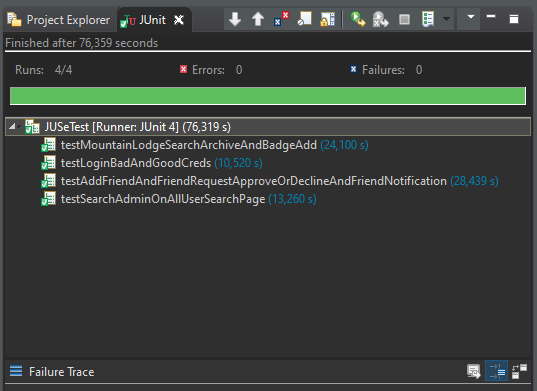
\includegraphics[scale=0.6, height=65mm, width=100mm]{slike/test_results.png} %veličina slike u odnosu na originalnu datoteku i pozicija slike
			\centering
			\caption{Uspješno izvršeni Selenium testovi - lokalno računalo}
			\label{fig:test_results}
		\end{figure}
		
			\eject 
		
		
		\section{Dijagram razmještaja}
			
			\textbf{\textit{dio 2. revizije}}
			
			 \textit{Potrebno je umetnuti \textbf{specifikacijski} dijagram razmještaja i opisati ga. Moguće je umjesto specifikacijskog dijagrama razmještaja umetnuti dijagram razmještaja instanci, pod uvjetom da taj dijagram bolje opisuje neki važniji dio sustava.}
			
			\eject 
		
		\section{Upute za puštanje u pogon}
		
			\textbf{\textit{dio 2. revizije}}\\
		
			 \textit{U ovom poglavlju potrebno je dati upute za puštanje u pogon (engl. deployment) ostvarene aplikacije. Na primjer, za web aplikacije, opisati postupak kojim se od izvornog kôda dolazi do potpuno postavljene baze podataka i poslužitelja koji odgovara na upite korisnika. Za mobilnu aplikaciju, postupak kojim se aplikacija izgradi, te postavi na neku od trgovina. Za stolnu (engl. desktop) aplikaciju, postupak kojim se aplikacija instalira na računalo. Ukoliko mobilne i stolne aplikacije komuniciraju s poslužiteljem i/ili bazom podataka, opisati i postupak njihovog postavljanja. Pri izradi uputa preporučuje se \textbf{naglasiti korake instalacije uporabom natuknica} te koristiti što je više moguće \textbf{slike ekrana} (engl. screenshots) kako bi upute bile jasne i jednostavne za slijediti.}
			
			
			 \textit{Dovršenu aplikaciju potrebno je pokrenuti na javno dostupnom poslužitelju. Studentima se preporuča korištenje neke od sljedećih besplatnih usluga: \href{https://aws.amazon.com/}{Amazon AWS}, \href{https://azure.microsoft.com/en-us/}{Microsoft Azure} ili \href{https://www.heroku.com/}{Heroku}. Mobilne aplikacije trebaju biti objavljene na F-Droid, Google Play ili Amazon App trgovini.}
			
			
			\eject 